\section{Simulations}\label{sec:sims}

This section uses Monte Carlo to compare three data-driven choices of the shrinkage intensity $\alpha$: the Ledoit--Wolf intensity, the Gaussian SURE of Section~\ref{sec:stein}, and the distribution-free SURE of Section~\ref{sec:df-sure}. The main question is what happens when the data are not normal. The Gaussian SURE relies on normal fourth moments, so under heavy tails it should misjudge $\operatorname{Var}(s_{ij})$. The distribution-free SURE estimates the fourth moments directly and should stay unbiased. All code is in \texttt{sims/sim\_section6.py}. Every experiment uses its own fixed seed, and the whole script runs in about two minutes.
% TODO(Jack): add RBLW/OAS (Chen et al. 2010) and Touloumis (2015) if citation approved

\subsection{Setup}

Each replication draws $x_1, \dots, x_T \in \mathbb{R}^N$ i.i.d.\ with mean zero and covariance $\Sigma$. It forms $S = \frac{1}{T}\sum_{t=1}^T x_t x_t'$ and the target $F = \nu I$ with $\nu = \operatorname{tr}(S)/N$. It then evaluates $\hat\Sigma = \alpha F + (1-\alpha) S$ under the loss $\|\hat\Sigma - \Sigma\|^2$ (squared Frobenius norm).

\paragraph{Distributions.} We use three data models, all with $\operatorname{Cov}(x_t) = \Sigma$:
\begin{itemize}
  \item Gaussian: $x_t \sim N(0, \Sigma)$.
  \item Multivariate $t$ with $\kappa$ degrees of freedom: $x_t = \sqrt{w_t}\, z_t$ with $z_t \sim N(0, \Sigma)$ and $w_t = (\kappa - 2)/\chi^2_\kappa$ independent of $z_t$, so that $\mathbb{E} w_t = 1$. We use $\kappa = 10$ and, as a stress test, $\kappa = 5$.
\end{itemize}
For the $t$ model, $\mathbb{E}\|x_t\|^4 = \frac{\kappa - 2}{\kappa - 4}\left[ (\operatorname{tr}\Sigma)^2 + 2\operatorname{tr}(\Sigma^2) \right]$. This is $4/3$ times the Gaussian value for $\kappa = 10$ and $3$ times for $\kappa = 5$. Fourth moments are finite in both cases, so the estimators of Section~\ref{sec:df-sure} are unbiased. Eighth moments, however, are finite only for $\kappa > 8$. With $\kappa = 5$ the estimates $\hat V$ and $\hat C$, and the losses themselves, have infinite variance, and plain Monte Carlo averages settle slowly. The next paragraphs explain how we handle this.

\paragraph{Covariance matrices.} We use two choices of $\Sigma$:
\begin{itemize}
  \item Single-factor: $\Sigma = \sigma_m^2 \beta\beta' + \operatorname{diag}(d_1, \dots, d_N)$ with $\sigma_m^2 = 1$. The betas and the residual variances are both equally spaced on $[0.5, 1.5]$, in the same order, so the asset with the largest beta also has the largest residual variance. This is the market model of \citet{sharpe1963}, a natural structure for stock returns. One large eigenvalue makes $\Sigma$ far from $\nu I$, so the optimal intensity is small.
  \item Spread eigenvalues: $\Sigma = \operatorname{diag}(\lambda_1, \dots, \lambda_N)$ with $\lambda_i$ equally spaced on $[1, 10]$. Both data models are elliptical and the loss is invariant under rotations, so taking $\Sigma$ diagonal loses no generality. Here $\Sigma$ is much closer to $\nu I$ and the optimal intensity is large.
\end{itemize}

\paragraph{Design.} We cross $N \in \{10, 50, 100\}$ with $T \in \{20, 60, 250\}$, which gives $N/T$ from $0.04$ to $5$. We do this for each of the $2 \times 3$ combinations of $\Sigma$ and distribution, which makes 54 cells. Gaussian and $t_{10}$ cells use 5{,}000 replications each. Each $t_5$ cell is run 10 times independently with 5{,}000 replications per run, and we report the pooled result over all 50{,}000.

\subsection{Estimators}

All three intensities share the denominator $\|F - S\|^2 = \operatorname{tr}(S^2) - (\operatorname{tr}S)^2/N$.

\begin{enumerate}
  \item \emph{Ledoit--Wolf.} For the target $\nu I$, the intensity of \citet{ledoit2004} can be written as $\hat\alpha_{\mathrm{LW}} = \frac{T-1}{T}\, \hat V / \|F - S\|^2$, where $\hat V$ is the distribution-free estimate below (Section~\ref{sec:df-sure}). The code checks this identity numerically against the original formula.
  \item \emph{Gaussian SURE (Section~\ref{sec:stein}).}
  \[
    \hat V_G = \frac{T(\operatorname{tr}S)^2 + (T-2)\operatorname{tr}(S^2)}{(T+2)(T-1)}, \quad
    \hat b = \frac{T\left[ T\operatorname{tr}(S^2) - (\operatorname{tr}S)^2 \right]}{(T+2)(T-1)}, \quad
    \hat\alpha_G = \frac{\hat V_G - 2\hat b/(NT)}{\|F - S\|^2}.
  \]
  \item \emph{Distribution-free SURE (Section~\ref{sec:df-sure}).} With $\hat M = \frac{1}{T}\sum_t \|x_t\|^4$, $\hat U_2 = \frac{1}{T(T-1)}\sum_{t \ne u}(x_t'x_u)^2$ and $\hat U_3 = \frac{1}{T(T-1)}\sum_{t \ne u}\|x_t\|^2\|x_u\|^2$,
  \[
    \hat V = \frac{\hat M - \hat U_2}{T}, \qquad
    \hat C = \frac{\hat M - \hat U_3}{NT}, \qquad
    \hat\alpha_{\mathrm{DF}} = \frac{\hat V - \hat C}{\|F - S\|^2}.
  \]
  \item \emph{Oracle.} $\alpha^* = (V - C)/D$, where
  \[
    V = \sum_{i,j}\operatorname{Var}(s_{ij}) = \frac{\mathbb{E}\|x_t\|^4 - \operatorname{tr}(\Sigma^2)}{T}, \qquad
    C = \sum_{i,j}\operatorname{Cov}(f_{ij}, s_{ij}) = \frac{\mathbb{E}\|x_t\|^4 - (\operatorname{tr}\Sigma)^2}{NT},
  \]
  and $D = \mathbb{E}\|F - S\|^2$, all known in closed form. The oracle minimizes the true risk $R(\alpha) = \alpha^2 D + (1 - 2\alpha)V + 2\alpha C$ over constant $\alpha$ and uses the unknown $\Sigma$.
\end{enumerate}
The sample covariance $S$ ($\alpha = 0$) is the baseline. Every intensity is clipped to $[0, 1]$. Across all cells, clipping was needed for 0.63\% of LW draws, 0.04\% of Gaussian SURE draws and 1.66\% of distribution-free SURE draws.

Under normality the two SURE versions agree in expectation. There $\mathbb{E}\|x_t\|^4 = (\operatorname{tr}\Sigma)^2 + 2\operatorname{tr}(\Sigma^2)$, and the targets of $\hat V$ and $\hat C$ reduce to those of $\hat V_G$ and $2\hat b/(NT)$. The two versions differ only in how they estimate the fourth moment.

\paragraph{Performance measure.} We report the percentage relative improvement in average loss over $S$,
\[
  \mathrm{PRIAL} = 100 \times \frac{\mathbb{E}\|S - \Sigma\|^2 - \mathbb{E}\|\hat\Sigma - \Sigma\|^2}{\mathbb{E}\|S - \Sigma\|^2}.
\]
The denominator is known exactly, $\mathbb{E}\|S - \Sigma\|^2 = V$, and so is the oracle's numerator, $V - R(\alpha^*) = (V - C)^2/D$ when $\alpha^* \in [0,1]$. The oracle PRIAL is therefore exact, $100(V - C)^2/(DV)$. For the data-driven methods we estimate $\mathbb{E}\|\hat\Sigma - \Sigma\|^2$ by Monte Carlo. We use $L_S = \|S - \Sigma\|^2$, whose mean $V$ is known, as a control variate: the plain average of the loss is corrected by $\hat\beta(\bar L_S - V)$, where $\hat\beta$ is the regression slope of the loss on $L_S$. This matters for $t_5$. There a few samples with an extreme day produce huge losses, and without the correction single-run PRIALs swing by tens of points. With the correction, the run-to-run standard deviation of a single 5{,}000-replication $t_5$ PRIAL is at most $1.7$ points for LW and the distribution-free SURE, and at most $0.7$ points for the Gaussian SURE.

\paragraph{Monte Carlo error.} The standard error of a single PRIAL is at most $0.64$ points in the Gaussian cells and $0.66$ points in the $t_{10}$ cells, and it is much smaller in most cells. All methods are evaluated on the same replications, so differences between methods are more precise than the levels. The standard error of the difference between the two SUREs is at most $0.17$ points in the Gaussian cells and $0.59$ points in the $t_{10}$ cells. The standard error of the difference between LW and the distribution-free SURE is at most $0.03$ points. Every cell's standard errors are listed in \texttt{sims/out/sec6\_results.txt}.

\subsection{Results}

\paragraph{The risk curve.} Figure~\ref{fig:sec6-curves} shows the two SURE curves averaged over 20{,}000 replications, for the single-factor $\Sigma$ with $N = 100$ and $T = 20$, next to the true risk $R(\alpha)$. Under normality all three curves coincide: both averages are within 0.5\% of $R(0)$ at every $\alpha \in [0,1]$. Under $t_{10}$ the distribution-free curve is still on target (within 0.8\%). The Gaussian curve, however, is shifted down by up to 26\% of $R(0)$. Its value at $\alpha = 0$ estimates $V = \mathbb{E}\|S - \Sigma\|^2$, and the Gaussian formula misses the extra kurtosis. Its minimizer therefore sits to the left of $\alpha^*$.

\begin{figure}[htbp]
  \centering
  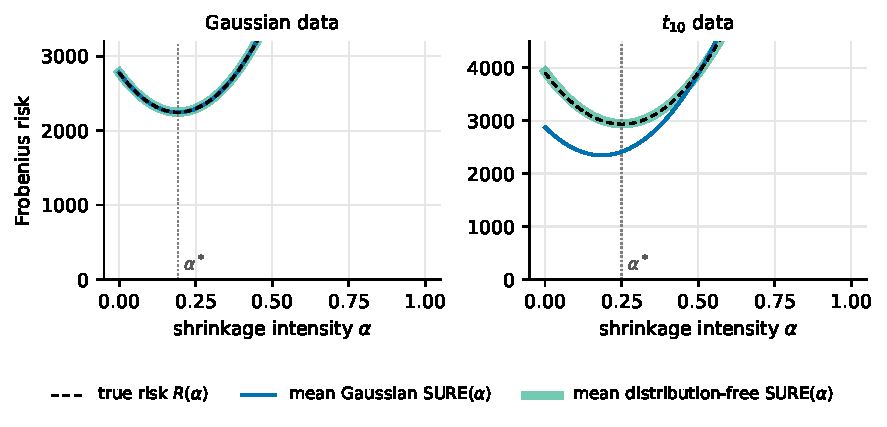
\includegraphics[width=\linewidth]{sec6_sure_curves}
  \caption{Mean SURE$(\alpha)$ over 20{,}000 replications against the true risk $R(\alpha)$. Single-factor $\Sigma$, $N = 100$, $T = 20$, shown for $\alpha \in [0, 0.6]$. In the Gaussian panel the three curves coincide. Dotted vertical line: $\alpha^*$.}
  \label{fig:sec6-curves}
\end{figure}

\paragraph{Bias of the variance terms.} Table~\ref{tab:sec6-bias} shows the source of the shift. Under normality all four estimates are unbiased.
\begin{itemize}
  \item Under $t_{10}$, $\hat V_G$ captures only about three quarters of $V$, and $2\hat b/(NT)$ captures between 15\% and 56\% of $C$. The covariance term is hit hardest: with heavy tails, $C$ contains a $(\operatorname{tr}\Sigma)^2$ term that the Gaussian formula $2\operatorname{tr}(\Sigma^2)/(NT)$ does not have.
  \item Under $t_5$, $\hat V_G$ falls to under 40\% of $V$.
\end{itemize}
The distribution-free estimates are within 2\% of the truth under $t_{10}$. Under $t_5$ their Monte Carlo means range from 0.83 to 1.04 even with 50{,}000 replications. This does not contradict unbiasedness, which needs only fourth moments. With infinite eighth moments, the average of $\hat V$ is dominated by rare large draws and settles slowly.

\begin{table}[htbp]
  \centering
  \caption{Monte Carlo mean of each estimate divided by its true value ($1$ means unbiased). $N = 100$, $T = 20$. There are 5{,}000 replications per row, except 50{,}000 for $t_5$.}
  \label{tab:sec6-bias}
  \begin{tabular}{llcccc}
    \toprule
    $\Sigma$ & data & $\hat V_G / V$ & $\hat V / V$ & $\frac{2\hat b/(NT)}{C}$ & $\hat C / C$ \\
    \midrule
    single-factor & Gaussian & 1.01 & 1.00 & 1.01 & 1.00 \\
                  & $t_{10}$ & 0.74 & 1.01 & 0.56 & 1.02 \\
                  & $t_5$    & 0.36 & 1.03 & 0.23 & 1.04 \\
    \midrule
    spread        & Gaussian & 1.00 & 1.00 & 1.00 & 1.00 \\
                  & $t_{10}$ & 0.77 & 1.00 & 0.15 & 1.00 \\
                  & $t_5$    & 0.38 & 0.88 & 0.09 & 0.83 \\
    \bottomrule
  \end{tabular}
\end{table}

\paragraph{Shrinkage intensities and PRIAL.} Table~\ref{tab:sec6-main} reports results for $N = 100$. Figure~\ref{fig:sec6-prial} shows the PRIAL in all 54 cells, and Figure~\ref{fig:sec6-alpha} shows the error of $\hat\alpha$ in the 27 single-factor cells. The full table is in \texttt{sims/out/sec6\_results.txt}.

\begin{table}[htbp]
  \centering
  \small
  \setlength{\tabcolsep}{4pt}
  \caption{Mean shrinkage intensity and PRIAL (\%) for $N = 100$. G = Gaussian SURE, DF = distribution-free SURE. Oracle PRIAL is exact; the other PRIALs use 5{,}000 replications per row, or 50{,}000 for $t_5$.}
  \label{tab:sec6-main}
  \begin{tabular}{llrcccccrrrr}
    \toprule
    & & & & \multicolumn{3}{c}{mean $\hat\alpha$} & & \multicolumn{4}{c}{PRIAL (\%)} \\
    \cmidrule(lr){5-7} \cmidrule(lr){9-12}
    $\Sigma$ & data & $T$ & $\alpha^*$ & LW & G & DF & & LW & G & DF & Oracle \\
    \midrule
    single-factor & Gaussian & 20  & 0.191 & 0.205 & 0.215 & 0.215 & & 10.5 & 10.7 & 10.0 & 19.1 \\
                  &          & 60  & 0.073 & 0.076 & 0.077 & 0.076 & & 3.4  & 3.4  & 3.4  & 7.3 \\
                  &          & 250 & 0.019 & 0.019 & 0.019 & 0.019 & & 0.1  & 0.1  & 0.1  & 1.8 \\
                  & $t_{10}$ & 20  & 0.249 & 0.252 & 0.215 & 0.264 & & 20.5 & 14.4 & 20.2 & 24.8 \\
                  &          & 60  & 0.100 & 0.099 & 0.076 & 0.100 & & 8.8  & 5.1  & 8.8  & 9.9 \\
                  &          & 250 & 0.026 & 0.026 & 0.019 & 0.026 & & 2.9  & 1.4  & 2.9  & 2.6 \\
                  & $t_5$    & 20  & 0.447 & 0.318 & 0.208 & 0.332 & & 57.5 & 19.0 & 57.6 & 44.4 \\
                  &          & 60  & 0.213 & 0.149 & 0.076 & 0.150 & & 43.1 & 7.5  & 43.1 & 21.1 \\
                  &          & 250 & 0.061 & 0.047 & 0.019 & 0.046 & & 27.5 & 2.0  & 27.4 & 6.0 \\
    \midrule
    spread        & Gaussian & 20  & 0.957 & 0.909 & 0.957 & 0.957 & & 95.4 & 95.6 & 95.6 & 95.7 \\
                  &          & 60  & 0.881 & 0.867 & 0.881 & 0.881 & & 88.0 & 88.0 & 88.0 & 88.1 \\
                  &          & 250 & 0.640 & 0.638 & 0.640 & 0.640 & & 63.9 & 63.9 & 63.9 & 64.0 \\
                  & $t_{10}$ & 20  & 0.967 & 0.920 & 0.778 & 0.965 & & 96.2 & 90.0 & 96.4 & 96.5 \\
                  &          & 60  & 0.908 & 0.894 & 0.704 & 0.907 & & 90.5 & 84.6 & 90.5 & 90.6 \\
                  &          & 250 & 0.703 & 0.701 & 0.531 & 0.702 & & 70.2 & 65.5 & 70.2 & 70.2 \\
                  & $t_5$    & 20  & 0.985 & 0.930 & 0.610 & 0.974 & & 97.7 & 56.5 & 97.9 & 97.9 \\
                  &          & 60  & 0.957 & 0.924 & 0.500 & 0.935 & & 95.1 & 50.1 & 95.1 & 95.1 \\
                  &          & 250 & 0.842 & 0.799 & 0.364 & 0.798 & & 84.5 & 42.2 & 84.5 & 83.7 \\
    \bottomrule
  \end{tabular}
\end{table}

\begin{figure}[htbp]
  \centering
  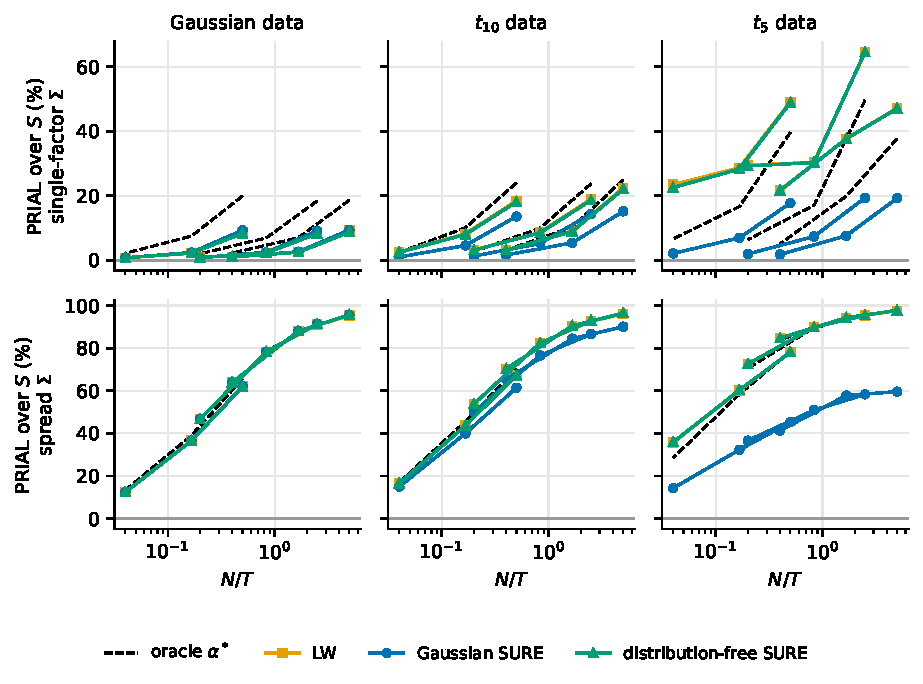
\includegraphics[width=\linewidth]{sec6_prial}
  \caption{PRIAL over $S$ against $N/T$ (log scale) for all 54 cells. Points with the same $N$ are joined; within each joined set, $T = 250, 60, 20$ from left to right. The markers are nested (large hollow square for LW, hollow circle for the Gaussian SURE, small filled triangle for the distribution-free SURE), so methods that coincide stay visible. Top row: single-factor $\Sigma$. Bottom row: spread eigenvalues.}
  \label{fig:sec6-prial}
\end{figure}

\begin{figure}[htbp]
  \centering
  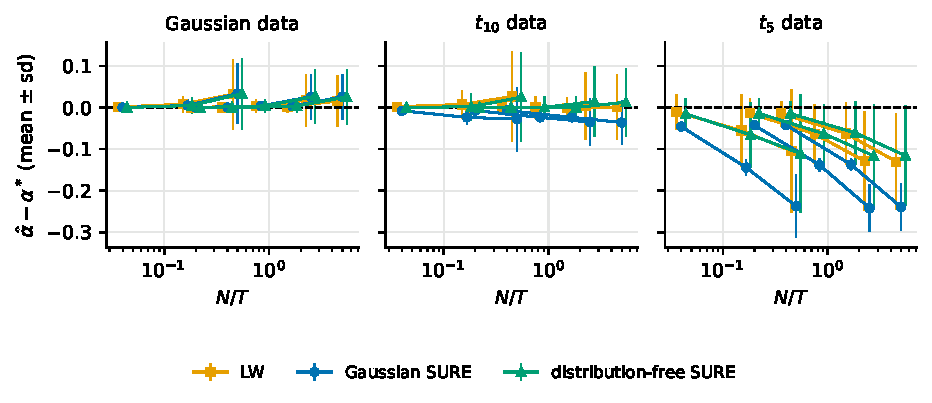
\includegraphics[width=\linewidth]{sec6_alpha}
  \caption{Mean of $\hat\alpha - \alpha^*$ (markers) with $\pm 1$ standard deviation of $\hat\alpha$ (bars), for the 27 single-factor cells. Points with the same $N$ are joined, and markers are offset horizontally for readability.}
  \label{fig:sec6-alpha}
\end{figure}

Four findings stand out.

\begin{enumerate}
  \item \emph{Under normality the three methods are nearly identical.} Their PRIALs differ by at most $1.0$ point. The Gaussian SURE is slightly better for the single-factor $\Sigma$ at $T = 20$ ($10.7$ against $10.0$ at $N = 100$, a difference of about five standard errors). This is because its $\hat\alpha$ has a smaller standard deviation ($0.051$ against $0.062$). Using a known fourth-moment formula is more efficient when that formula is correct, and estimating the fourth moment from the data costs a little variance.
  \item \emph{Under $t_{10}$ the Gaussian SURE under-shrinks, and the distribution-free SURE does not.} The mean $\hat\alpha_G$ is $12$--$27\%$ below $\alpha^*$ for the single-factor $\Sigma$ and $16$--$25\%$ below for the spread $\Sigma$. The mean $\hat\alpha_{\mathrm{DF}}$ stays within $0.02$ of $\alpha^*$. The distribution-free SURE gains $1.4$--$6.4$ PRIAL points over the Gaussian SURE, and every one of these differences is at least nine paired standard errors. In the single-factor case this is a large share of the available gain ($20.2$ against $14.4$ at $N = 100$, $T = 20$, with the oracle at $24.8$).
  \item \emph{Under $t_5$ the gap becomes severe.} The Gaussian SURE achieves only $32$--$58\%$ of the oracle's improvement and trails LW and the distribution-free SURE by at least $23$ points in every cell. LW and the distribution-free SURE shrink less than $\alpha^*$ on average, but they match or beat the oracle. The effect is most visible for the single-factor $\Sigma$, where they beat the oracle by $11$--$22$ points in all nine cells. It also appears for the spread $\Sigma$ at $N = 10$ ($40.7$ against $30.5$ at $T = 250$) and at $N = 50$, $T = 250$. A weak version appears under $t_{10}$ at $T = 250$. For the single-factor $\Sigma$, LW and the distribution-free SURE are $0.1$--$0.3$ points above the oracle, which is within one standard error. For the spread $\Sigma$ they are within $0.4$ points of it.

  Beating the oracle is possible because $\alpha^*$ is optimal only among constants. A data-dependent $\hat\alpha$ can shrink more in exactly the samples where $S$ is far from $\Sigma$. A separate run with 200{,}000 replications (single-factor $\Sigma$, $N = 100$, $T = 20$, $t_5$) shows how. One huge day makes $S$ nearly rank one, $\|F - S\|^2$ and $\hat V$ are then both dominated by that day, and $\hat\alpha_{\mathrm{LW}}$ moves toward one. In the 0.1\% of samples with the largest $\|S - \Sigma\|^2$ the mean $\hat\alpha_{\mathrm{LW}}$ is $0.80$, against $0.26$ in the half with the smallest. These 0.1\% of samples supply 45\% of LW's total reduction in loss relative to $S$. Overall the paired difference is $\mathbb{E}[L(\mathrm{LW}) - L(\alpha^*)] = -0.25\,R(\alpha^*)$ (standard error $0.06\,R(\alpha^*)$).
  \item \emph{LW and the distribution-free SURE are almost indistinguishable in this design.} Their PRIALs differ by at most $0.9$ points in every cell. LW shrinks visibly less only when $N/T$ is large and $\alpha^*$ is near one, as in the spread $\Sigma$, Gaussian, $N = 100$, $T = 20$ cell (mean $0.909$ against $0.957$). Even there the PRIAL difference is $0.2$ points. Starting from $\hat V$, LW subtracts $\hat V/T$ (the factor $(T-1)/T$), while SURE subtracts $\hat C$ (Section~\ref{sec:df-sure}). Under normality $C/V \le 1/N$, so the SURE correction is at most about $\hat V/N$. Its size relative to the LW correction varies widely: $\hat C$ is about $13$ times $\hat V/T$ in the single-factor Gaussian cell with $N = 10$, $T = 250$. In this design, however, both corrections are small next to $\hat V$, because $T \ge 20$ and $N \ge 10$.
\end{enumerate}

A further point concerns the gap to the oracle. Under normality, in the single-factor case at $T = 20$, the oracle PRIAL ($19$) is about twice that of every data-driven method ($7$--$11$). Here $\alpha^*$ is small and $D$ is large, so the noise in $\hat\alpha$ (standard deviation about $0.05$--$0.08$, against $\alpha^* \approx 0.19$) costs a large share of the possible gain. All three methods also over-shrink slightly on average (about $0.22$ against $0.19$). This matches the remark in Section~\ref{sec:df-sure}: SURE is unbiased for the risk curve, but its minimizer, a ratio of estimates, is not unbiased for $\alpha^*$. Under heavy tails the gap to the oracle narrows (under $t_{10}$) or reverses (under $t_5$), as described above.

\subsection{Discussion}

The simulations support the theory of Sections~\ref{sec:stein} and~\ref{sec:df-sure}. Under normality both SURE versions estimate the risk curve without bias and pick nearly the same intensity. When the data have fatter tails than the normal, the Gaussian SURE underestimates $\operatorname{Var}(s_{ij})$ and, even more, $\operatorname{Cov}(f_{ij}, s_{ij})$. It shrinks too little and loses a sizeable part of the improvement over $S$. The distribution-free SURE stays on target. Heavy tails are commonly reported for daily stock returns. If they are present in the application that motivates this thesis, the distribution-free version is the safer choice. Its cost is a small loss of efficiency when the data really are normal.

The comparison with Ledoit--Wolf is less decisive. For $T \ge 20$ the LW intensity is within a fraction of a PRIAL point of the distribution-free SURE. This agrees with the identity $\hat\alpha_{\mathrm{LW}} = \frac{T-1}{T}\hat V/\|F - S\|^2$: LW already uses the same distribution-free estimate of $\operatorname{Var}(s_{ij})$, and the two methods differ only in a small correction to $\hat V$. In this range of $T$ the advantage of the SURE derivation over LW is therefore mostly conceptual. It gives an exactly unbiased risk estimate rather than an asymptotic one. Whether SURE also gives a practical advantage at much smaller $T$ is not tested here.

Two limitations apply. First, the mean is known to be zero throughout; with a demeaned sample covariance the identities used here hold only approximately. Second, all data models are elliptical. Skewed or non-elliptical returns, and returns that are dependent over time, are not covered.
